\section{速度場の計算}

\begin{figure}
	\centering
	
	\begin{minipage}[b]{0.2\linewidth}
		\centering
		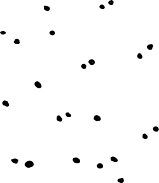
\includegraphics[width=\linewidth]{./pic/outflow_ex1.png}
		\subcaption{}
		\label{}
	\end{minipage}
	\begin{minipage}[b]{0.2\linewidth}
		\centering
		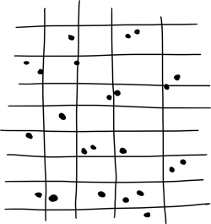
\includegraphics[width=\linewidth]{./pic/outflow_ex2.png}
		\subcaption{}
		\label{}
	\end{minipage} 
	\begin{minipage}[b]{0.2\linewidth}
		\centering
		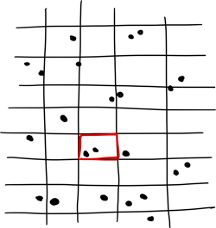
\includegraphics[width=\linewidth]{./pic/outflow_ex3.png}
		\subcaption{}
		\label{}
	\end{minipage}
	\begin{minipage}[b]{0.2\linewidth}
		\centering
		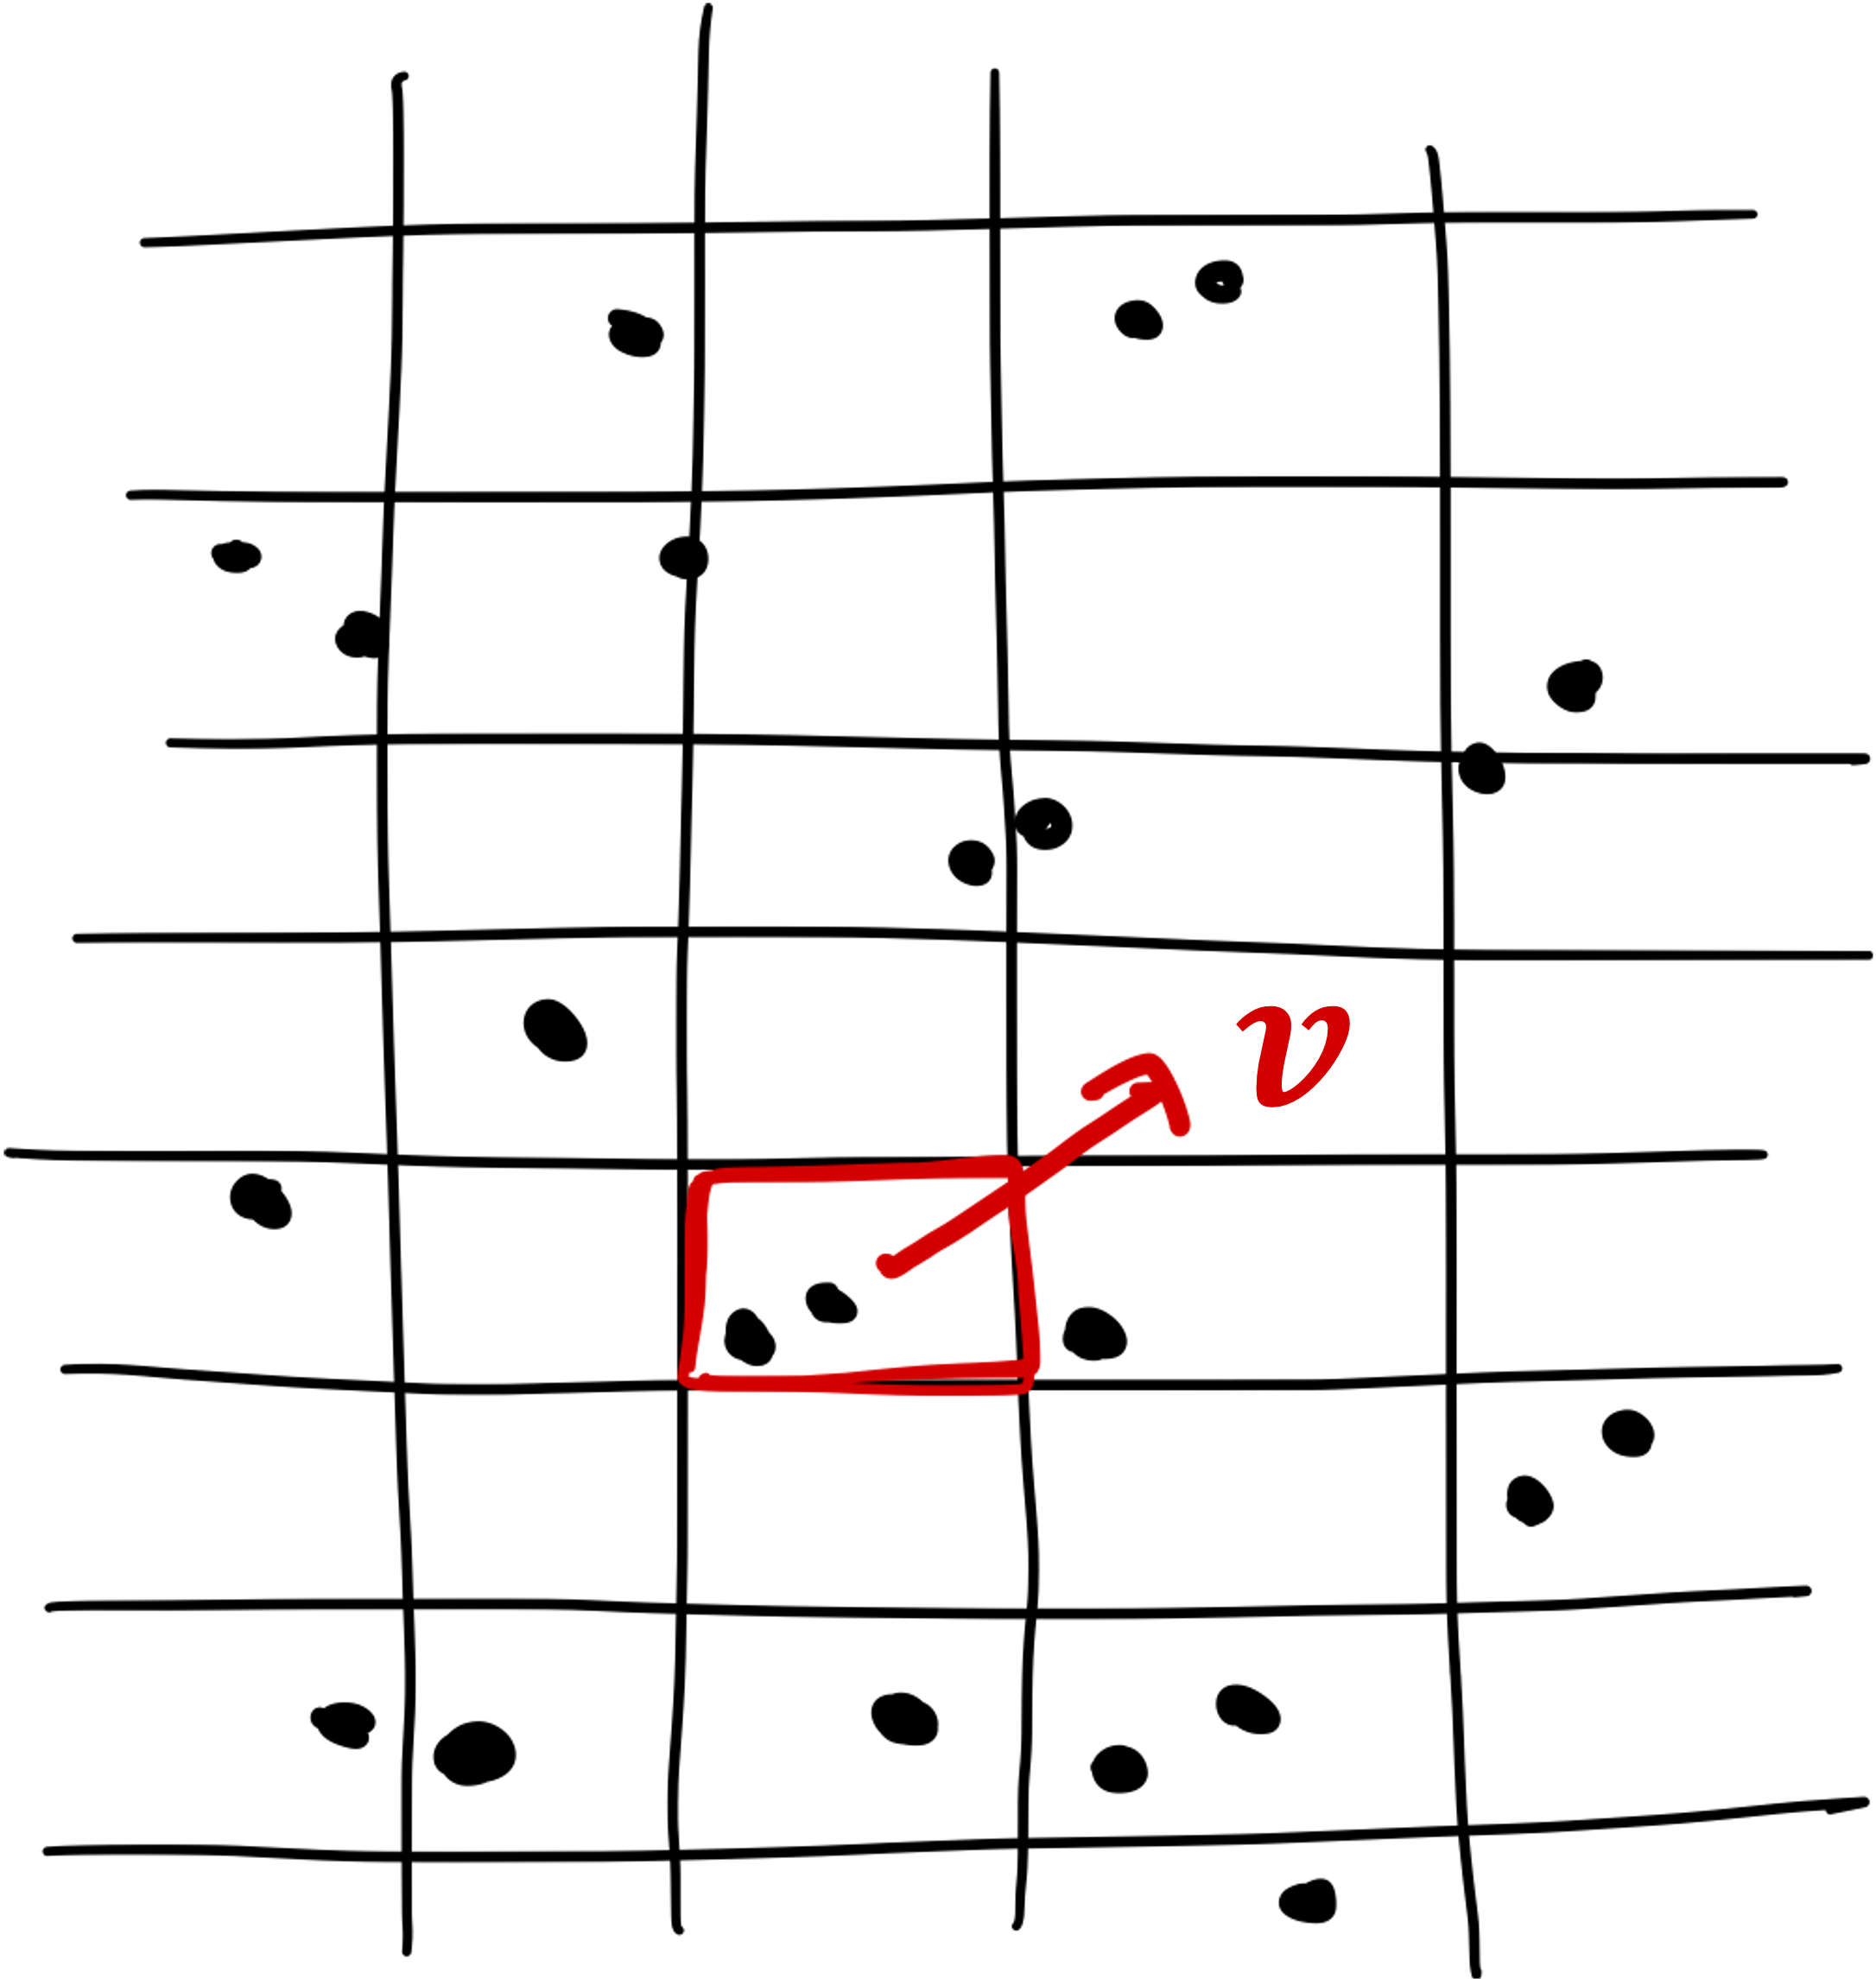
\includegraphics[width=\linewidth]{./pic/outflow_ex4.png}
		\subcaption{}
		\label{}
	\end{minipage}
	\begin{minipage}[b]{\linewidth}
		\centering
		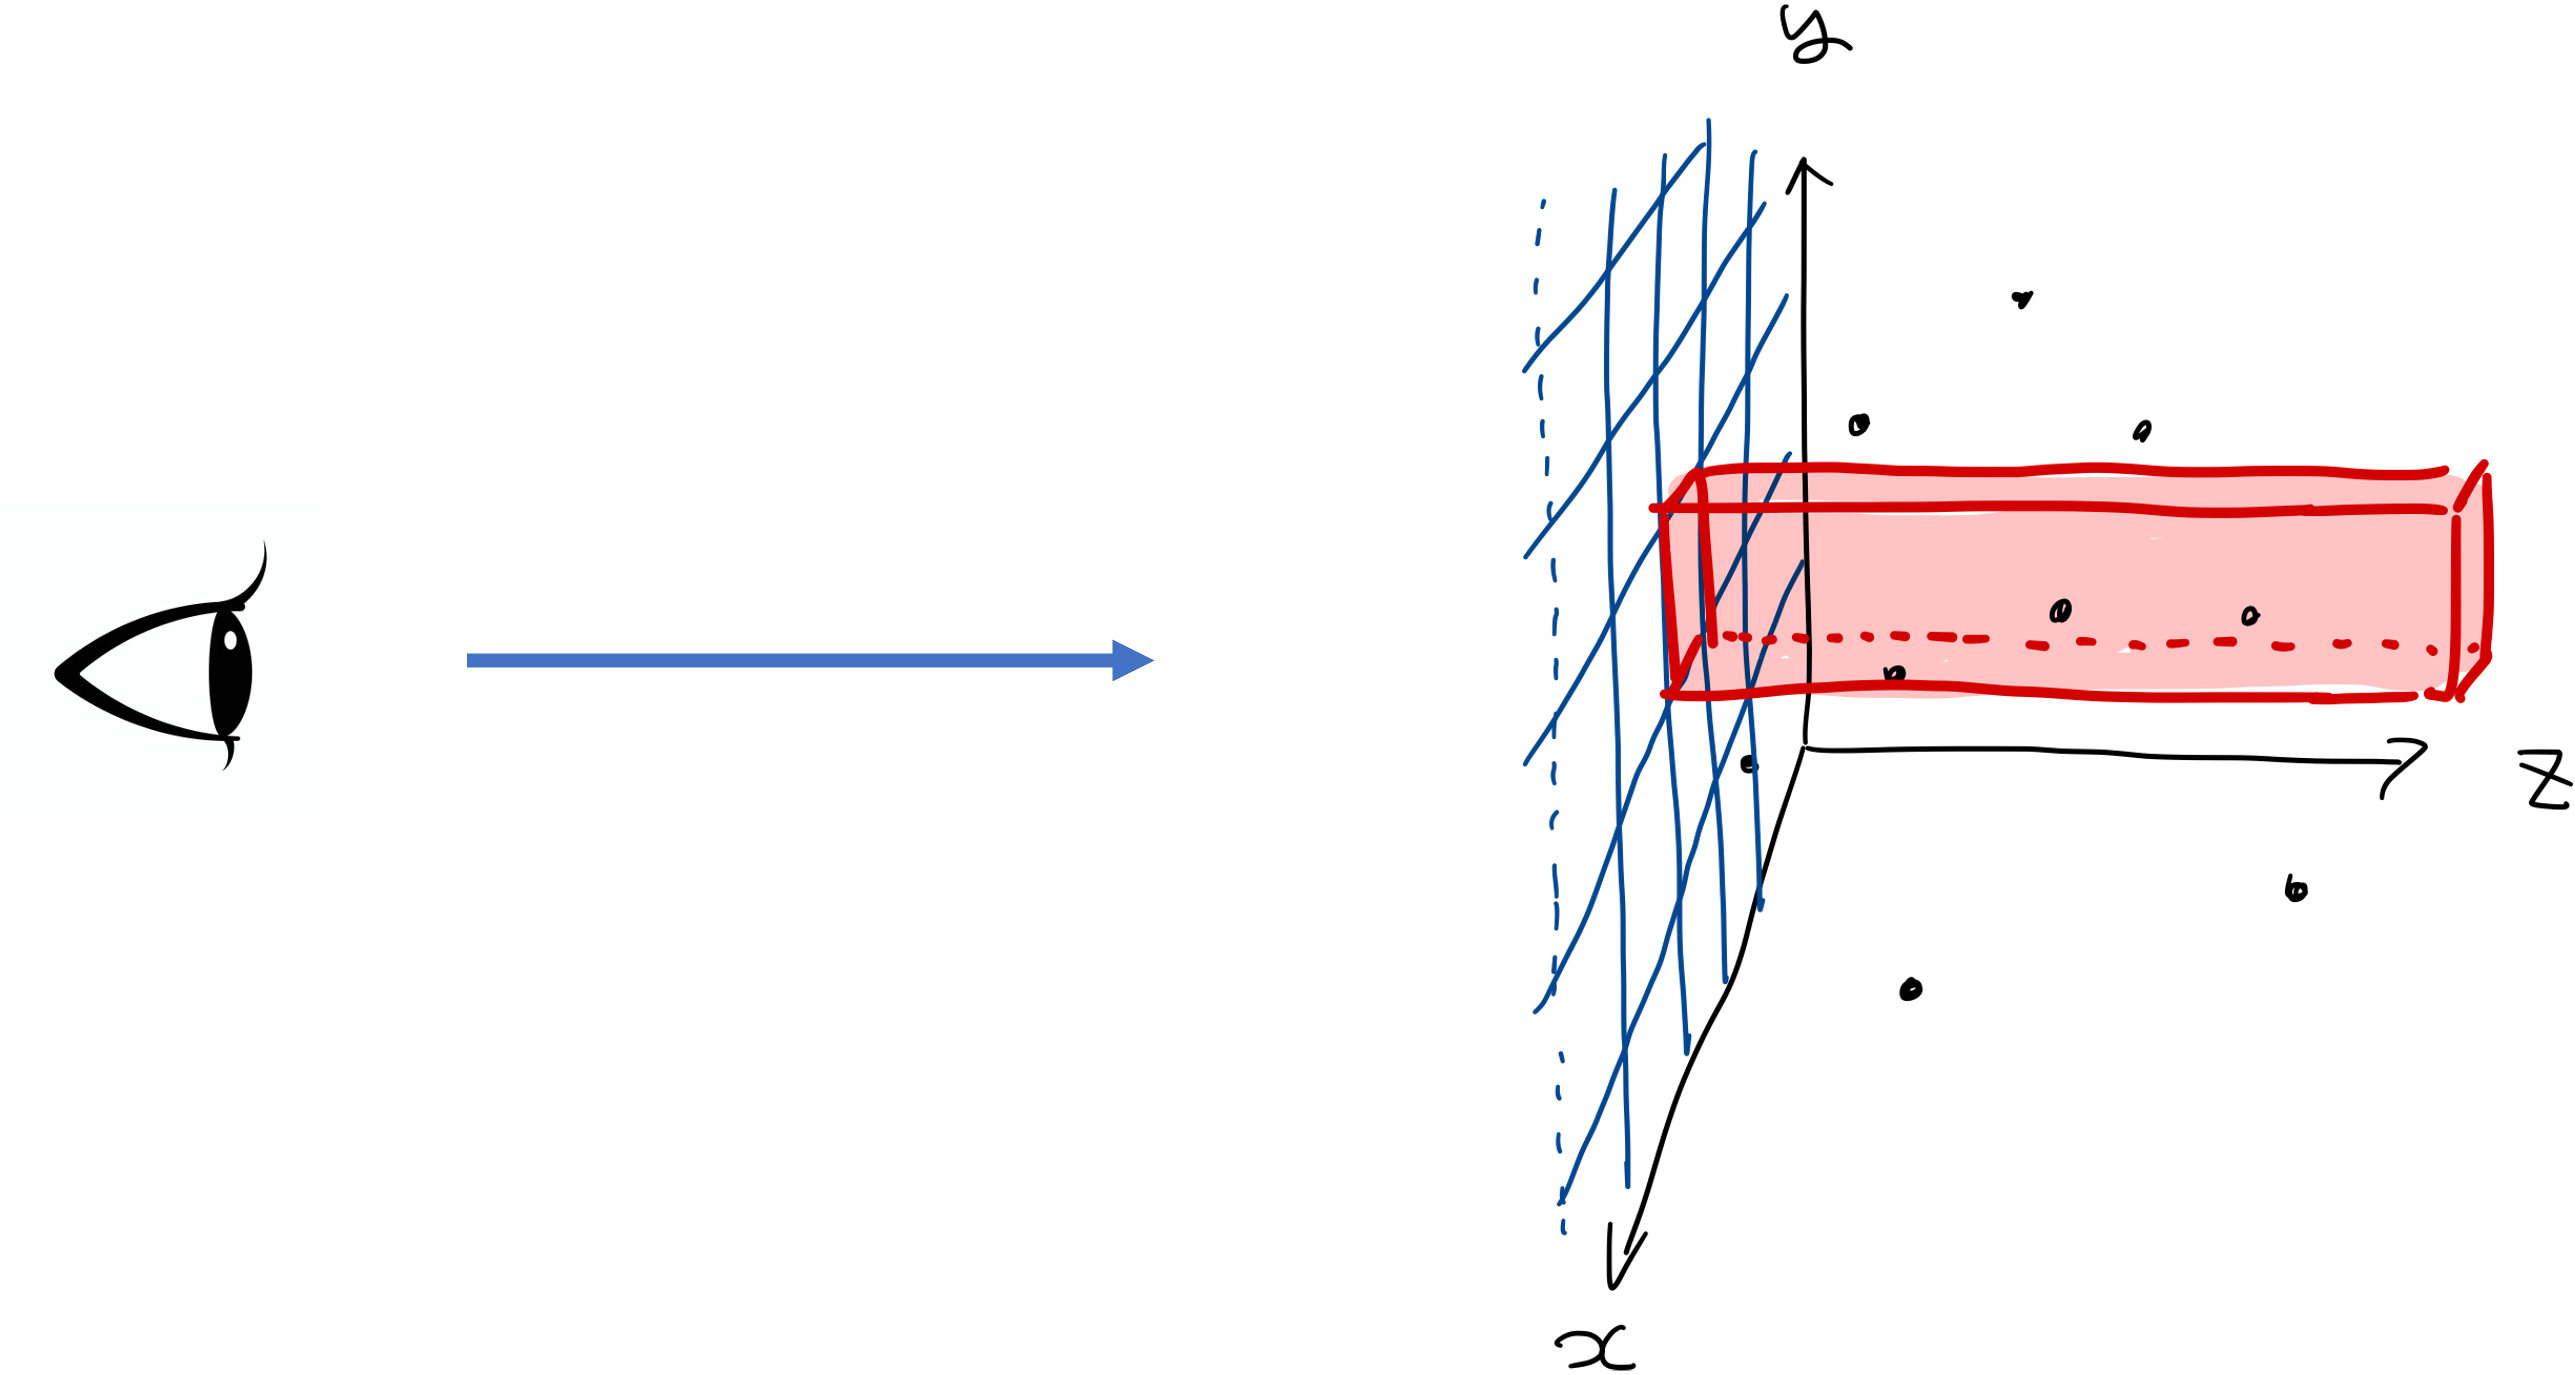
\includegraphics[width=0.55\linewidth]{./pic/outflow_ex5.png}
		\subcaption{}
		\label{}
	\end{minipage}
	
	\caption{(a)シミュレーションデータ内には粒子/メッシュが存在する,(b)$x$,$y$に対してビンまとめを行う,(c)ビンまとめをしたらビン内の平均速度を導出する,}
	\label{}
\end{figure}